\section{Theoretical Background}

\subsection{What is being measured in this lab?}
In this experiment, you are measuring \emph{head loss}, which is the loss of mechanical energy of the flowing fluid between two locations in the system. In pipe flow, head loss is caused by two broad mechanisms:

\begin{itemize}[leftmargin=*]
    \item \textbf{Major losses:} frictional losses distributed along the wall of a straight pipe over a finite length.
    \item \textbf{Minor losses:} local losses caused by fittings or abrupt geometry changes such as valves, elbows, sudden contractions, sudden expansions, venturis, and orifices.
\end{itemize}

The purpose of this lab is to compare measured head losses to theoretical predictions for both of these mechanisms, and to understand how flow rate, roughness, diameter, and fittings affect the result.

\subsection{Laminar, Transitional, and Turbulent Flow}
The first step in most pipe-flow calculations is to identify the flow regime using the Reynolds number:
\begin{equation}
Re = \frac{\rho \bar{V} D}{\mu}
\label{eq:reynolds}
\end{equation}
where:
\begin{itemize}[leftmargin=*]
    \item \(\rho\) is the fluid density \((\mathrm{kg/m^3})\),
    \item \(\bar{V}\) is the mean velocity \((\mathrm{m/s})\),
    \item \(D\) is the internal pipe diameter \((\mathrm{m})\),
    \item \(\mu\) is the dynamic viscosity \((\mathrm{Pa\cdot s})\).
\end{itemize}

For internal pipe flow, the usual classification is:
\begin{center}
\begin{tabular}{cc}
\toprule
Reynolds Number & Flow Regime \\
\midrule
\(Re < 2100\) & Laminar \\
\(2100 < Re < 4000\) & Transitional \\
\(Re > 4000\) & Turbulent \\
\bottomrule
\end{tabular}
\end{center}

This classification appears in the lab material and is specifically for pipe flow. The velocity profile is strongly influenced by the flow regime: laminar flow gives a parabolic profile, while turbulent flow produces a much flatter time-averaged profile with steep gradients near the wall.

\begin{figure}[H]
    \centering
    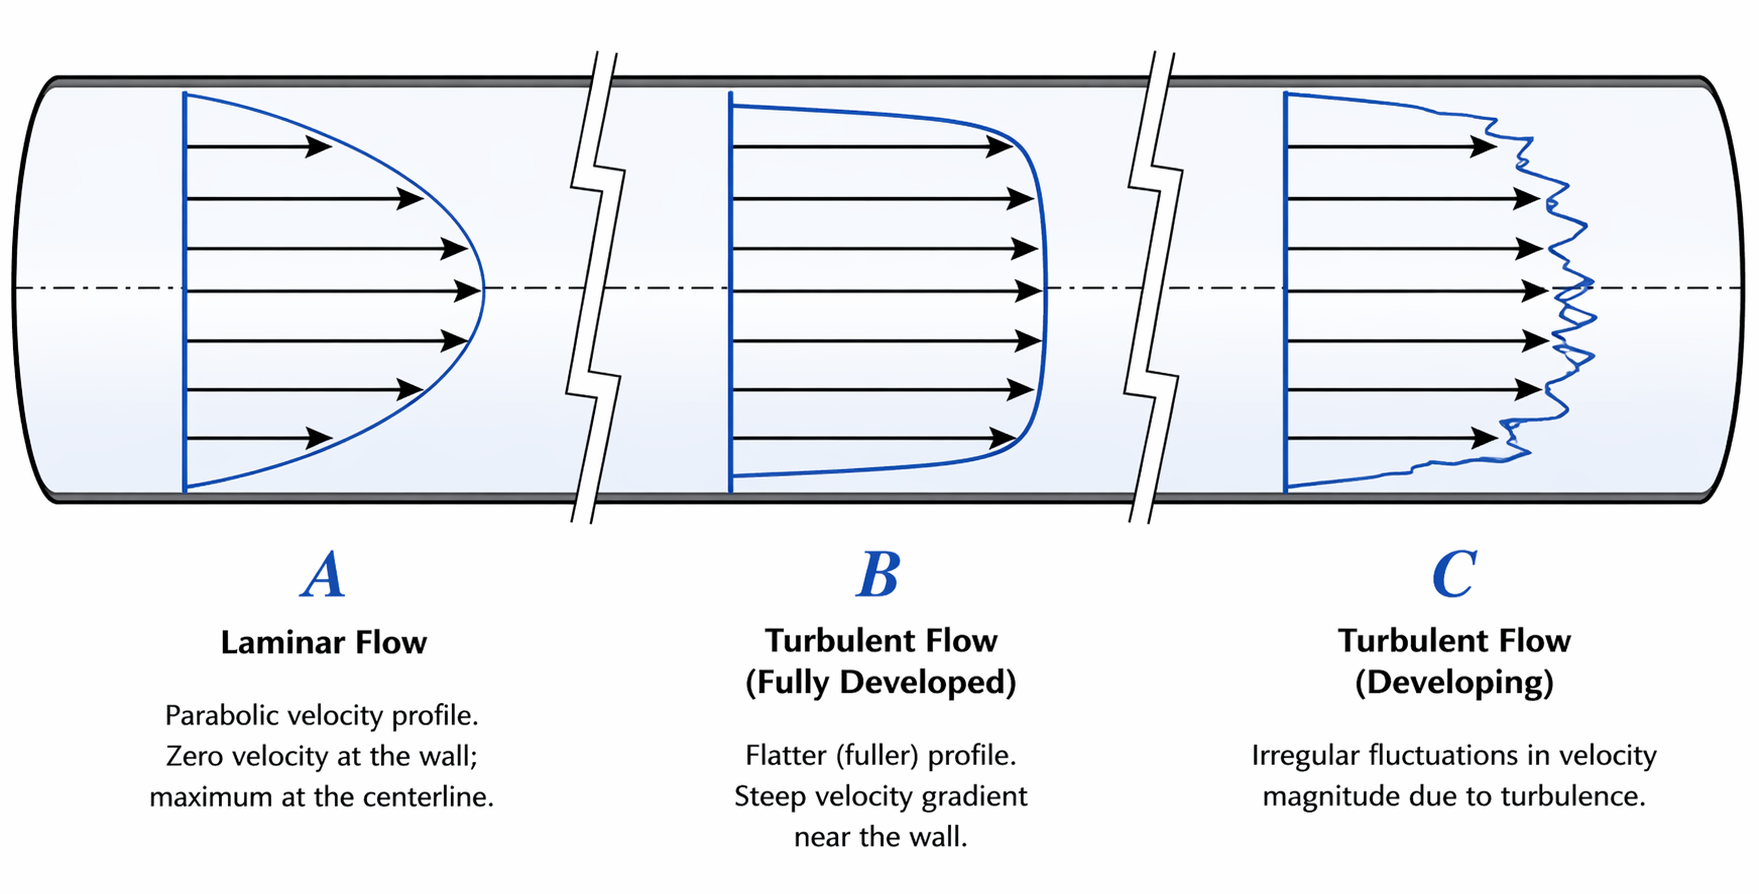
\includegraphics[width=0.82\textwidth]{Lab2_Figures/Vel_profile_updated.png}
    \caption{Velocity profiles for laminar and turbulent pipe flow.}
    \label{fig:velocity-profiles}
\end{figure}

\subsection{Flow Rate, Area, and Continuity}
The mean velocity and volumetric flow rate are related by
\begin{equation}
Q = \bar{V}A
\label{eq:flowrate}
\end{equation}
For a circular pipe,
\begin{equation}
A = \frac{\pi D^2}{4}
\end{equation}
so that
\begin{equation}
\bar{V} = \frac{Q}{A} = \frac{4Q}{\pi D^2}
\label{eq:velocityfromQ}
\end{equation}

Conservation of mass requires
\begin{equation}
Q_1 = Q_2
\qquad \Longrightarrow \qquad
\bar{V}_1 A_1 = \bar{V}_2 A_2
\label{eq:continuity}
\end{equation}
Thus, if the cross-sectional area changes, the average velocity must change inversely.

\subsection{Bernoulli Equation with Head Loss}
The Bernoulli equation between two points along a streamline is
\begin{equation}
\frac{p_1}{\rho g} + \frac{\bar{V}_1^2}{2g} + z_1
=
\frac{p_2}{\rho g} + \frac{\bar{V}_2^2}{2g} + z_2 + h_L
\label{eq:bernoulli-loss}
\end{equation}
where \(h_L\) is the total head loss between points 1 and 2.

The total head loss is split into
\begin{equation}
h_L = h_{L,\text{major}} + h_{L,\text{minor}}
\label{eq:headlosssum}
\end{equation}

\subsubsection*{Important simplification for this lab}
Many segments in this apparatus are horizontal and have constant diameter. In that case,
\[
z_1=z_2
\qquad \text{and} \qquad
\bar{V}_1=\bar{V}_2
\]
so Eq.~\eqref{eq:bernoulli-loss} simplifies to
\begin{equation}
h_L = \frac{p_1-p_2}{\rho g}
\label{eq:horizontal-head-loss}
\end{equation}

This is one of the most important working equations in the lab. It explains why a measured pressure difference across a straight, level, constant-diameter segment can be interpreted directly as a head loss.
\noindent
\textit{Note: The constant-diameter simplification above applies to the
3--2 portion of Figure~\ref{fig:headlosssimple}; the diameter change between
points 2 and 1 requires use of the full energy equation, Eq.~\eqref{eq:bernoulli-loss}.}
\begin{figure}[H]
    \centering
    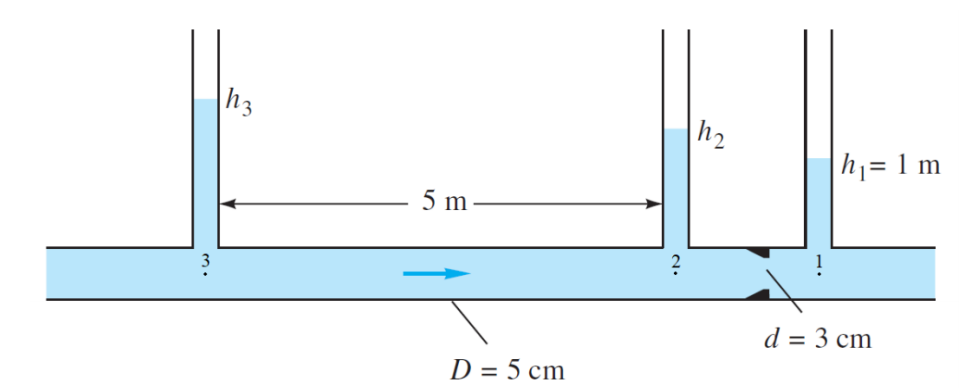
\includegraphics[width=0.82\textwidth]{Lab2_Figures/manometer.png}
    \caption{Depiction of head loss in a simple horizontal pipe section.}
    \label{fig:headlosssimple}
\end{figure}

\subsection{Major Head Loss: Darcy--Weisbach Equation}
For straight-pipe friction over a length \(L\), the major head loss is
\begin{equation}
h_{L,\text{major}} = f\frac{L}{D}\frac{\bar{V}^2}{2g}
\label{eq:darcy}
\end{equation}
where \(f\) is the Darcy friction factor.

\subsubsection*{Laminar flow}
For fully developed laminar flow,
\begin{equation}
f = \frac{64}{Re}
\label{eq:laminarf}
\end{equation}

\subsubsection*{Turbulent flow: implicit and explicit formulas}
For turbulent flow, \(f\) depends on both Reynolds number and relative roughness \(\varepsilon/D\).

The standard implicit relation is the Colebrook--White equation:
\begin{equation}
\frac{1}{\sqrt{f}}
=
-2.0\log_{10}
\left(
\frac{\varepsilon/D}{3.7}
+
\frac{2.51}{Re\sqrt{f}}
\right)
\label{eq:colebrook}
\end{equation}

Because Eq.~\eqref{eq:colebrook} is implicit in \(f\), explicit approximations are often preferred for hand calculations and spreadsheets.

\paragraph{Haaland equation}
A convenient explicit approximation is
\begin{equation}
\frac{1}{\sqrt{f}}
\approx
-1.8\log_{10}
\left[
\left(
\frac{\varepsilon/D}{3.7}
\right)^{1.11}
+
\frac{6.9}{Re}
\right]
\label{eq:haaland}
\end{equation}

\paragraph{Swamee--Jain equation}
Another widely used explicit approximation is
\begin{equation}
f
\approx
0.25
\left[
\log_{10}
\left(
\frac{\varepsilon/D}{3.7}
+
\frac{5.74}{Re^{0.9}}
\right)
\right]^{-2}
\label{eq:swameejain}
\end{equation}

For most turbulent pipe-flow calculations in this course, using Haaland or Swamee--Jain is an efficient alternative to iterating Colebrook or reading directly from the Moody chart.

\subsubsection*{Recommended friction-factor workflow}
For student calculations, the following workflow is recommended:
\begin{enumerate}[leftmargin=*]
    \item Compute \(Q\), \(A\), and \(\bar{V}\).
    \item Compute \(Re\).
    \item If \(Re < 2100\), use Eq.~\eqref{eq:laminarf}.
    \item If \(Re > 4000\), compute \(f\) using Eq.~\eqref{eq:haaland} or Eq.~\eqref{eq:swameejain}.
    \item Optionally cross-check the result against the Moody chart using \(Re\) and \(\varepsilon/D\).
\end{enumerate}

\subsection{Minor Head Loss}
A minor loss due to a fitting is written as
\begin{equation}
h_{L,\text{minor}} = K_L \frac{\bar{V}^2}{2g}
\label{eq:minor}
\end{equation}
where \(K_L\) is the loss coefficient and \(\bar{V}\) is usually the largest relevant mean velocity associated with the fitting.

For this lab, the following correlations are used:

\begin{table}[H]
\centering
\caption{Pipe fittings and their loss-coefficient equations}
\label{tab:KL}
\small
\begingroup
\setlength{\tabcolsep}{4pt}
\begin{tabular}{m{0.17\textwidth} m{0.66\textwidth}}
\toprule
Fitting & Loss coefficient equation \\
\midrule
Elbow at \(90^\circ\) &
ITO equation (turbulent regime):
\[
\begin{aligned}
K_L ={}& 0.367\left(\frac{r}{D}\right)^{-0.84} \\
&+ 1.71\left(\frac{r}{D}\right)^{-1.11}Re^{-0.17}
\end{aligned}
\]
where \(r\) is the radius of curvature of the elbow. \\[1em]

Orifice &
Gibson equation:
\[
K_L = 2.8\left(1-\frac{d}{D}\right)^2
\left[\left(\frac{D}{d}\right)^2 -1\right]
\]
where \(d\) is the orifice diameter. \\[1em]

Sudden expansion &
Carnot equation:
\[
K_L = \left(1-\left(\frac{d}{D}\right)^2\right)^2
\]
where \(d\) is the smaller and \(D\) is the larger diameter. \\[1em]

Sudden contraction &
\[
K_L = 0.42\left(1-\left(\frac{d}{D}\right)^2\right)
\]
where \(d\) is the smaller and \(D\) is the larger diameter. \\
\bottomrule
\end{tabular}
\endgroup
\end{table}

\subsection{How to treat fittings carefully in Bernoulli calculations}
For fittings, do \textbf{not} automatically cancel the kinetic-energy terms. If the diameter changes across the fitting, then \(\bar{V}_1 \neq \bar{V}_2\), and Eq.~\eqref{eq:bernoulli-loss} must be used in full:
\[
\frac{p_1}{\rho g} + \frac{\bar{V}_1^2}{2g} + z_1
=
\frac{p_2}{\rho g} + \frac{\bar{V}_2^2}{2g} + z_2 + h_L
\]
This is especially important for the venturi, orifice, sudden contraction, and sudden expansion.

\subsection{Instrument conversions used in the lab}
Measured pressure differences are often reported in mbar or as manometer height differences. Convert carefully:
\begin{itemize}[leftmargin=*]
    \item DPT reading in mbar \(\rightarrow\) Pa using \(1~\mathrm{mbar}=100~\mathrm{Pa}\)
    \item Pressure difference \(\Delta p\) to head loss using
    \[
    h_L = \frac{\Delta p}{\rho g}
    \]
    \item For water, a manometer reading in mm-H\(_2\)O is already a head difference, so
    \[
    h_L = \Delta h
    \]
    after converting mm to m
\end{itemize}

\subsection{What students should do in each part}
\paragraph{Part 1: Manometer vs DPT}
Use Eq.~\eqref{eq:horizontal-head-loss} to convert both measurements into head loss and compare the instruments directly.

\paragraph{Part 2: Major losses}
Use Eq.~\eqref{eq:darcy} with the appropriate friction factor:
\begin{itemize}[leftmargin=*]
    \item laminar: Eq.~\eqref{eq:laminarf}
    \item turbulent: Eq.~\eqref{eq:haaland} or Eq.~\eqref{eq:swameejain}
\end{itemize}
Then compare theory to measured \(h_L\).

\paragraph{Part 3: Minor losses}
Compute \(K_L\)-based minor losses using Eq.~\eqref{eq:minor}, and include any velocity-head change if the diameter changes.

\paragraph{Part 4: Effect of flow rate}
Since \(\bar{V}\propto Q\), both major and minor losses scale roughly with \(Q^2\) once the friction factor is relatively stable. Thus the measured \(h_L\)-vs-\(Q\) curve should generally be nonlinear and often close to quadratic over the turbulent range.